% Options for packages loaded elsewhere
\PassOptionsToPackage{unicode}{hyperref}
\PassOptionsToPackage{hyphens}{url}
\PassOptionsToPackage{dvipsnames,svgnames,x11names}{xcolor}
%
\documentclass[
  letterpaper,
  DIV=11]{scrreprt}

\usepackage{amsmath,amssymb}
\usepackage{lmodern}
\usepackage{iftex}
\ifPDFTeX
  \usepackage[T1]{fontenc}
  \usepackage[utf8]{inputenc}
  \usepackage{textcomp} % provide euro and other symbols
\else % if luatex or xetex
  \usepackage{unicode-math}
  \defaultfontfeatures{Scale=MatchLowercase}
  \defaultfontfeatures[\rmfamily]{Ligatures=TeX,Scale=1}
\fi
% Use upquote if available, for straight quotes in verbatim environments
\IfFileExists{upquote.sty}{\usepackage{upquote}}{}
\IfFileExists{microtype.sty}{% use microtype if available
  \usepackage[]{microtype}
  \UseMicrotypeSet[protrusion]{basicmath} % disable protrusion for tt fonts
}{}
\makeatletter
\@ifundefined{KOMAClassName}{% if non-KOMA class
  \IfFileExists{parskip.sty}{%
    \usepackage{parskip}
  }{% else
    \setlength{\parindent}{0pt}
    \setlength{\parskip}{6pt plus 2pt minus 1pt}}
}{% if KOMA class
  \KOMAoptions{parskip=half}}
\makeatother
\usepackage{xcolor}
\setlength{\emergencystretch}{3em} % prevent overfull lines
\setcounter{secnumdepth}{3}
% Make \paragraph and \subparagraph free-standing
\ifx\paragraph\undefined\else
  \let\oldparagraph\paragraph
  \renewcommand{\paragraph}[1]{\oldparagraph{#1}\mbox{}}
\fi
\ifx\subparagraph\undefined\else
  \let\oldsubparagraph\subparagraph
  \renewcommand{\subparagraph}[1]{\oldsubparagraph{#1}\mbox{}}
\fi

\usepackage{color}
\usepackage{fancyvrb}
\newcommand{\VerbBar}{|}
\newcommand{\VERB}{\Verb[commandchars=\\\{\}]}
\DefineVerbatimEnvironment{Highlighting}{Verbatim}{commandchars=\\\{\}}
% Add ',fontsize=\small' for more characters per line
\usepackage{framed}
\definecolor{shadecolor}{RGB}{241,243,245}
\newenvironment{Shaded}{\begin{snugshade}}{\end{snugshade}}
\newcommand{\AlertTok}[1]{\textcolor[rgb]{0.68,0.00,0.00}{#1}}
\newcommand{\AnnotationTok}[1]{\textcolor[rgb]{0.37,0.37,0.37}{#1}}
\newcommand{\AttributeTok}[1]{\textcolor[rgb]{0.40,0.45,0.13}{#1}}
\newcommand{\BaseNTok}[1]{\textcolor[rgb]{0.68,0.00,0.00}{#1}}
\newcommand{\BuiltInTok}[1]{\textcolor[rgb]{0.00,0.23,0.31}{#1}}
\newcommand{\CharTok}[1]{\textcolor[rgb]{0.13,0.47,0.30}{#1}}
\newcommand{\CommentTok}[1]{\textcolor[rgb]{0.37,0.37,0.37}{#1}}
\newcommand{\CommentVarTok}[1]{\textcolor[rgb]{0.37,0.37,0.37}{\textit{#1}}}
\newcommand{\ConstantTok}[1]{\textcolor[rgb]{0.56,0.35,0.01}{#1}}
\newcommand{\ControlFlowTok}[1]{\textcolor[rgb]{0.00,0.23,0.31}{#1}}
\newcommand{\DataTypeTok}[1]{\textcolor[rgb]{0.68,0.00,0.00}{#1}}
\newcommand{\DecValTok}[1]{\textcolor[rgb]{0.68,0.00,0.00}{#1}}
\newcommand{\DocumentationTok}[1]{\textcolor[rgb]{0.37,0.37,0.37}{\textit{#1}}}
\newcommand{\ErrorTok}[1]{\textcolor[rgb]{0.68,0.00,0.00}{#1}}
\newcommand{\ExtensionTok}[1]{\textcolor[rgb]{0.00,0.23,0.31}{#1}}
\newcommand{\FloatTok}[1]{\textcolor[rgb]{0.68,0.00,0.00}{#1}}
\newcommand{\FunctionTok}[1]{\textcolor[rgb]{0.28,0.35,0.67}{#1}}
\newcommand{\ImportTok}[1]{\textcolor[rgb]{0.00,0.46,0.62}{#1}}
\newcommand{\InformationTok}[1]{\textcolor[rgb]{0.37,0.37,0.37}{#1}}
\newcommand{\KeywordTok}[1]{\textcolor[rgb]{0.00,0.23,0.31}{#1}}
\newcommand{\NormalTok}[1]{\textcolor[rgb]{0.00,0.23,0.31}{#1}}
\newcommand{\OperatorTok}[1]{\textcolor[rgb]{0.37,0.37,0.37}{#1}}
\newcommand{\OtherTok}[1]{\textcolor[rgb]{0.00,0.23,0.31}{#1}}
\newcommand{\PreprocessorTok}[1]{\textcolor[rgb]{0.68,0.00,0.00}{#1}}
\newcommand{\RegionMarkerTok}[1]{\textcolor[rgb]{0.00,0.23,0.31}{#1}}
\newcommand{\SpecialCharTok}[1]{\textcolor[rgb]{0.37,0.37,0.37}{#1}}
\newcommand{\SpecialStringTok}[1]{\textcolor[rgb]{0.13,0.47,0.30}{#1}}
\newcommand{\StringTok}[1]{\textcolor[rgb]{0.13,0.47,0.30}{#1}}
\newcommand{\VariableTok}[1]{\textcolor[rgb]{0.07,0.07,0.07}{#1}}
\newcommand{\VerbatimStringTok}[1]{\textcolor[rgb]{0.13,0.47,0.30}{#1}}
\newcommand{\WarningTok}[1]{\textcolor[rgb]{0.37,0.37,0.37}{\textit{#1}}}

\providecommand{\tightlist}{%
  \setlength{\itemsep}{0pt}\setlength{\parskip}{0pt}}\usepackage{longtable,booktabs,array}
\usepackage{calc} % for calculating minipage widths
% Correct order of tables after \paragraph or \subparagraph
\usepackage{etoolbox}
\makeatletter
\patchcmd\longtable{\par}{\if@noskipsec\mbox{}\fi\par}{}{}
\makeatother
% Allow footnotes in longtable head/foot
\IfFileExists{footnotehyper.sty}{\usepackage{footnotehyper}}{\usepackage{footnote}}
\makesavenoteenv{longtable}
\usepackage{graphicx}
\makeatletter
\def\maxwidth{\ifdim\Gin@nat@width>\linewidth\linewidth\else\Gin@nat@width\fi}
\def\maxheight{\ifdim\Gin@nat@height>\textheight\textheight\else\Gin@nat@height\fi}
\makeatother
% Scale images if necessary, so that they will not overflow the page
% margins by default, and it is still possible to overwrite the defaults
% using explicit options in \includegraphics[width, height, ...]{}
\setkeys{Gin}{width=\maxwidth,height=\maxheight,keepaspectratio}
% Set default figure placement to htbp
\makeatletter
\def\fps@figure{htbp}
\makeatother
\newlength{\cslhangindent}
\setlength{\cslhangindent}{1.5em}
\newlength{\csllabelwidth}
\setlength{\csllabelwidth}{3em}
\newlength{\cslentryspacingunit} % times entry-spacing
\setlength{\cslentryspacingunit}{\parskip}
\newenvironment{CSLReferences}[2] % #1 hanging-ident, #2 entry spacing
 {% don't indent paragraphs
  \setlength{\parindent}{0pt}
  % turn on hanging indent if param 1 is 1
  \ifodd #1
  \let\oldpar\par
  \def\par{\hangindent=\cslhangindent\oldpar}
  \fi
  % set entry spacing
  \setlength{\parskip}{#2\cslentryspacingunit}
 }%
 {}
\usepackage{calc}
\newcommand{\CSLBlock}[1]{#1\hfill\break}
\newcommand{\CSLLeftMargin}[1]{\parbox[t]{\csllabelwidth}{#1}}
\newcommand{\CSLRightInline}[1]{\parbox[t]{\linewidth - \csllabelwidth}{#1}\break}
\newcommand{\CSLIndent}[1]{\hspace{\cslhangindent}#1}

\KOMAoption{captions}{tableheading}
\makeatletter
\makeatother
\makeatletter
\@ifpackageloaded{bookmark}{}{\usepackage{bookmark}}
\makeatother
\makeatletter
\@ifpackageloaded{caption}{}{\usepackage{caption}}
\AtBeginDocument{%
\ifdefined\contentsname
  \renewcommand*\contentsname{Inhaltsverzeichnis}
\else
  \newcommand\contentsname{Inhaltsverzeichnis}
\fi
\ifdefined\listfigurename
  \renewcommand*\listfigurename{Abbildungsverzeichnis}
\else
  \newcommand\listfigurename{Abbildungsverzeichnis}
\fi
\ifdefined\listtablename
  \renewcommand*\listtablename{Tabellenverzeichnis}
\else
  \newcommand\listtablename{Tabellenverzeichnis}
\fi
\ifdefined\figurename
  \renewcommand*\figurename{Abbildung}
\else
  \newcommand\figurename{Abbildung}
\fi
\ifdefined\tablename
  \renewcommand*\tablename{Tabelle}
\else
  \newcommand\tablename{Tabelle}
\fi
}
\@ifpackageloaded{float}{}{\usepackage{float}}
\floatstyle{ruled}
\@ifundefined{c@chapter}{\newfloat{codelisting}{h}{lop}}{\newfloat{codelisting}{h}{lop}[chapter]}
\floatname{codelisting}{Listing}
\newcommand*\listoflistings{\listof{codelisting}{Listingverzeichnis}}
\usepackage{amsthm}
\theoremstyle{definition}
\newtheorem{example}{Beispiel}[chapter]
\theoremstyle{remark}
\renewcommand*{\proofname}{Beweis}
\newtheorem*{remark}{Anmerkung}
\newtheorem*{solution}{Lösung}
\makeatother
\makeatletter
\@ifpackageloaded{caption}{}{\usepackage{caption}}
\@ifpackageloaded{subcaption}{}{\usepackage{subcaption}}
\makeatother
\makeatletter
\@ifpackageloaded{tcolorbox}{}{\usepackage[many]{tcolorbox}}
\makeatother
\makeatletter
\@ifundefined{shadecolor}{\definecolor{shadecolor}{rgb}{.97, .97, .97}}
\makeatother
\makeatletter
\makeatother
\ifLuaTeX
\usepackage[bidi=basic]{babel}
\else
\usepackage[bidi=default]{babel}
\fi
\babelprovide[main,import]{ngerman}
% get rid of language-specific shorthands (see #6817):
\let\LanguageShortHands\languageshorthands
\def\languageshorthands#1{}
\ifLuaTeX
  \usepackage{selnolig}  % disable illegal ligatures
\fi
\IfFileExists{bookmark.sty}{\usepackage{bookmark}}{\usepackage{hyperref}}
\IfFileExists{xurl.sty}{\usepackage{xurl}}{} % add URL line breaks if available
\urlstyle{same} % disable monospaced font for URLs
\hypersetup{
  pdftitle={AutoDiff},
  pdfauthor={Michael Brand},
  pdflang={de},
  colorlinks=true,
  linkcolor={blue},
  filecolor={Maroon},
  citecolor={Blue},
  urlcolor={Blue},
  pdfcreator={LaTeX via pandoc}}

\title{AutoDiff}
\usepackage{etoolbox}
\makeatletter
\providecommand{\subtitle}[1]{% add subtitle to \maketitle
  \apptocmd{\@title}{\par {\large #1 \par}}{}{}
}
\makeatother
\subtitle{Eine Einführung in algorithmisches Ableiten}
\author{Michael Brand}
\date{19/10/2022}

\begin{document}
\maketitle
\ifdefined\Shaded\renewenvironment{Shaded}{\begin{tcolorbox}[sharp corners, breakable, frame hidden, boxrule=0pt, borderline west={3pt}{0pt}{shadecolor}, enhanced, interior hidden]}{\end{tcolorbox}}\fi

\renewcommand*\contentsname{Inhaltsverzeichnis}
{
\hypersetup{linkcolor=}
\setcounter{tocdepth}{2}
\tableofcontents
}
\bookmarksetup{startatroot}

\hypertarget{vorwort}{%
\chapter*{Vorwort}\label{vorwort}}
\addcontentsline{toc}{chapter}{Vorwort}

\bookmarksetup{startatroot}

\hypertarget{einleitung}{%
\chapter*{Einleitung}\label{einleitung}}
\addcontentsline{toc}{chapter}{Einleitung}

\hypertarget{danksagung}{%
\section*{Danksagung}\label{danksagung}}
\addcontentsline{toc}{section}{Danksagung}

\bookmarksetup{startatroot}

\hypertarget{einfuxfchrung}{%
\chapter{Einführung}\label{einfuxfchrung}}

\bookmarksetup{startatroot}

\hypertarget{ad-ist-nicht}{%
\chapter{AD ist nicht \ldots{}}\label{ad-ist-nicht}}

Bevor wir uns mit den konkreten Implementationen von algorithmischer
Differentiation beschäftigen, wollen wir herausstellen, was AD
\emph{nicht} ist.

\hypertarget{ad-ist-nicht-numerisches-ableiten}{%
\section{AD ist nicht numerisches
Ableiten}\label{ad-ist-nicht-numerisches-ableiten}}

Eine Funktion \(y = f(x)\) ist bekanntlich differenzierbar an der Stelle
\(x_0 \in \mathbb{D}\), wenn der Grenzwert
\[ \lim_{h\rightarrow 0} \frac{f(x_0 + h) - f(x_0)}{h} \] existiert. In
dem Fall ist \(f'(x_0)\) einfach der Wert dieses Grenzwerts.

Ein erster Ansatz zur numerischen Berechnung könnte also sein, den
Differenzenquotienten für kleine \(h\) auszuwerten\footnote{Dieser
  Ansatz kann verbessert werden indem man z.B.
  \(f'(x_0) \approx \frac{f(x_0 + h) - f(x_0 - h)}{2h}\) verwendet. Die
  im Beispiel beschriebenen Probleme bleiben aber auch dann bestehen.}.

\leavevmode\vadjust pre{\hypertarget{exm-numDiff}{}}%
\begin{example}[Numerische Ableitung]\label{exm-numDiff}

Leite die Funktion \(f(x) = x^2\) an der Stelle \(x_0 = 2\) ab.

\begin{Shaded}
\begin{Highlighting}[]
\KeywordTok{def}\NormalTok{ f(x):}
\NormalTok{    y }\OperatorTok{=}\NormalTok{ x }\OperatorTok{**} \DecValTok{2}
    \ControlFlowTok{return}\NormalTok{ y}

\KeywordTok{def}\NormalTok{ fdot(f, x0, h):}
\NormalTok{    df }\OperatorTok{=}\NormalTok{ (f(x0 }\OperatorTok{+}\NormalTok{ h) }\OperatorTok{{-}}\NormalTok{ f(x0)) }\OperatorTok{/}\NormalTok{ h}
    \ControlFlowTok{return}\NormalTok{ df}

\NormalTok{x0 }\OperatorTok{=} \FloatTok{0.2}
\NormalTok{H }\OperatorTok{=}\NormalTok{ [}\FloatTok{0.1}\NormalTok{, }\FloatTok{0.01}\NormalTok{, }\FloatTok{0.001}\NormalTok{, }\FloatTok{0.0001}\NormalTok{]}
\ControlFlowTok{for}\NormalTok{ h }\KeywordTok{in}\NormalTok{ H:}
\NormalTok{    ydot }\OperatorTok{=}\NormalTok{ fdot(f, x0, h)}
    \BuiltInTok{print}\NormalTok{(}\StringTok{"h = "} \OperatorTok{+} \BuiltInTok{str}\NormalTok{(h) }\OperatorTok{+} \StringTok{" }\CharTok{\textbackslash{}t}\StringTok{=\textgreater{} f\textquotesingle{}(x0) = "} \OperatorTok{+} \BuiltInTok{str}\NormalTok{(ydot))}
\end{Highlighting}
\end{Shaded}

\begin{verbatim}
h = 0.1     => f'(x0) = 0.5000000000000001
h = 0.01    => f'(x0) = 0.4099999999999999
h = 0.001   => f'(x0) = 0.4009999999999986
h = 0.0001  => f'(x0) = 0.40009999999993107
\end{verbatim}

Es scheint zunächst, als ob die Werte für kleiner werdende \(h\) zum
korrekten Wert \(f'(0.2)=0.4\) konvergieren. Wenn wir aber an sehr
genauen Werten interessiert sind und entsprechen \(h\) sehr klein
wählen, beobachten wir folgendes:

\begin{Shaded}
\begin{Highlighting}[]
\KeywordTok{def}\NormalTok{ f(x):}
\NormalTok{    y }\OperatorTok{=}\NormalTok{ x }\OperatorTok{**} \DecValTok{2}
    \ControlFlowTok{return}\NormalTok{ y}

\KeywordTok{def}\NormalTok{ fdot(f, x0, h):}
\NormalTok{    df }\OperatorTok{=}\NormalTok{ (f(x0 }\OperatorTok{+}\NormalTok{ h) }\OperatorTok{{-}}\NormalTok{ f(x0)) }\OperatorTok{/}\NormalTok{ h}
    \ControlFlowTok{return}\NormalTok{ df}

\NormalTok{x0 }\OperatorTok{=} \FloatTok{0.2}
\NormalTok{H }\OperatorTok{=}\NormalTok{ [}\DecValTok{10} \OperatorTok{**} \OperatorTok{{-}}\DecValTok{8}\NormalTok{, }\DecValTok{10} \OperatorTok{**} \OperatorTok{{-}}\DecValTok{9}\NormalTok{, }\DecValTok{10} \OperatorTok{**} \OperatorTok{{-}}\DecValTok{10}\NormalTok{, }\DecValTok{10} \OperatorTok{**} \OperatorTok{{-}}\DecValTok{11}\NormalTok{]}
\ControlFlowTok{for}\NormalTok{ h }\KeywordTok{in}\NormalTok{ H:}
\NormalTok{    ydot }\OperatorTok{=}\NormalTok{ fdot(f, x0, h)}
    \BuiltInTok{print}\NormalTok{(}\StringTok{"h = "} \OperatorTok{+} \BuiltInTok{str}\NormalTok{(h) }\OperatorTok{+} \StringTok{"}\CharTok{\textbackslash{}t}\StringTok{=\textgreater{} f\textquotesingle{}(x0) = "} \OperatorTok{+} \BuiltInTok{str}\NormalTok{(ydot))}
\end{Highlighting}
\end{Shaded}

\begin{verbatim}
h = 1e-08   => f'(x0) = 0.4000000095039091
h = 1e-09   => f'(x0) = 0.3999999984016789
h = 1e-10   => f'(x0) = 0.4000000330961484
h = 1e-11   => f'(x0) = 0.3999994779846361
\end{verbatim}

Das Phänomen wird noch deutlicher, wenn wir den Fehler
\(E(h) = \lvert\frac{f(x_0+h)-f(x_0)}{h} - f'(x_0)\rvert\) als Funktion
von \(h\) plotten. Beachte die doppelt logarithmische Skala.

\begin{Shaded}
\begin{Highlighting}[]
\ImportTok{import}\NormalTok{ matplotlib.pyplot }\ImportTok{as}\NormalTok{ plt}
\ImportTok{import}\NormalTok{ math}

\KeywordTok{def}\NormalTok{ f(x):}
\NormalTok{    y }\OperatorTok{=}\NormalTok{ x }\OperatorTok{**} \DecValTok{2}
    \ControlFlowTok{return}\NormalTok{ y}

\KeywordTok{def}\NormalTok{ fdot(f, x0, h):}
\NormalTok{    df }\OperatorTok{=}\NormalTok{ (f(x0 }\OperatorTok{+}\NormalTok{ h) }\OperatorTok{{-}}\NormalTok{ f(x0)) }\OperatorTok{/}\NormalTok{ h}
    \ControlFlowTok{return}\NormalTok{ df}

\NormalTok{x0 }\OperatorTok{=} \FloatTok{0.2}
\NormalTok{H }\OperatorTok{=}\NormalTok{ [}\DecValTok{10}\OperatorTok{**}\NormalTok{(k}\OperatorTok{/}\DecValTok{100}\NormalTok{) }\ControlFlowTok{for}\NormalTok{ k }\KeywordTok{in} \BuiltInTok{range}\NormalTok{(}\OperatorTok{{-}}\DecValTok{1800}\NormalTok{, }\OperatorTok{{-}}\DecValTok{300}\NormalTok{)]}
\NormalTok{E }\OperatorTok{=}\NormalTok{ [math.fabs(fdot(f, x0, h) }\OperatorTok{{-}} \DecValTok{2}\OperatorTok{*}\NormalTok{x0) }\ControlFlowTok{for}\NormalTok{ h }\KeywordTok{in}\NormalTok{ H]}

\CommentTok{\# Plot}
\NormalTok{fig }\OperatorTok{=}\NormalTok{ plt.figure()}
\NormalTok{ax }\OperatorTok{=}\NormalTok{ fig.add\_axes([}\FloatTok{0.1}\NormalTok{, }\FloatTok{0.1}\NormalTok{, }\FloatTok{0.8}\NormalTok{, }\FloatTok{0.8}\NormalTok{])}
\NormalTok{ax.}\BuiltInTok{set}\NormalTok{(xlim}\OperatorTok{=}\NormalTok{(}\DecValTok{10}\OperatorTok{**{-}}\DecValTok{18}\NormalTok{, }\DecValTok{10}\OperatorTok{**{-}}\DecValTok{3}\NormalTok{), ylim}\OperatorTok{=}\NormalTok{(}\DecValTok{10}\OperatorTok{**{-}}\DecValTok{12}\NormalTok{, }\DecValTok{10}\OperatorTok{**}\DecValTok{0}\NormalTok{))}
\NormalTok{ax.set\_xscale(}\StringTok{\textquotesingle{}log\textquotesingle{}}\NormalTok{)}
\NormalTok{ax.set\_xlabel(}\StringTok{\textquotesingle{}h\textquotesingle{}}\NormalTok{)}
\NormalTok{ax.set\_yscale(}\StringTok{\textquotesingle{}log\textquotesingle{}}\NormalTok{)}
\NormalTok{ax.set\_ylabel(}\StringTok{\textquotesingle{}Fehler E(h)\textquotesingle{}}\NormalTok{)}
\NormalTok{plt.plot(H,E)}
\NormalTok{plt.show()}
\end{Highlighting}
\end{Shaded}

\begin{figure}[H]

{\centering 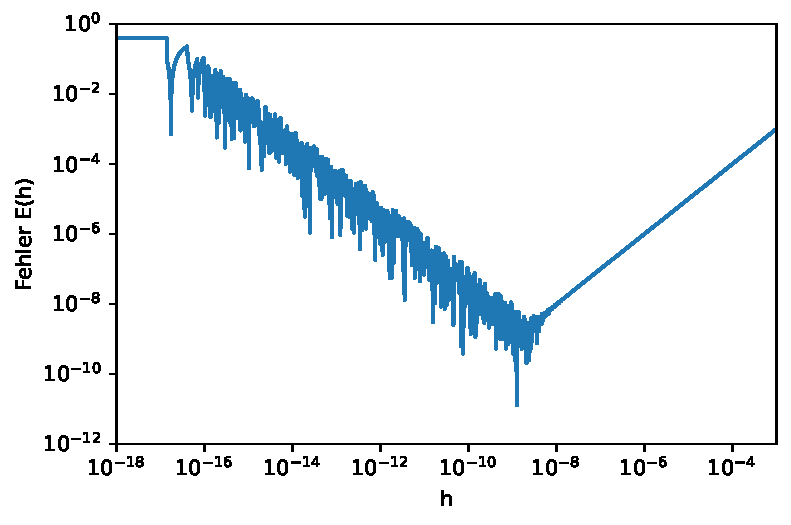
\includegraphics{./notAD_files/figure-pdf/fig-numdiffproblem-output-1.pdf}

}

\caption{\label{fig-numdiffproblem}Grösse des Fehlers \(E(h)\) als
Funktion der Schrittweite \(h\). Ist \(h\) zu gross, dann ist der
Näherungswert für \(f'(x_0)\) ungenau. Bei kleiner werdendem \(h\) nimmt
der Fehler zunächst ab, aber ab einem gewissen Wert dominiert die
Auslöschung und der Fehler nimmt wieder zu.}

\end{figure}

\begin{center}\rule{0.5\linewidth}{0.5pt}\end{center}

\end{example}

\hypertarget{ausluxf6schung}{%
\subsection{Auslöschung}\label{ausluxf6schung}}

Im vorherigen Beispiel haben wir das Phänomen der
\href{https://de.wikipedia.org/wiki/Ausl\%C3\%B6schung_(numerische_Mathematik)}{Auslöschung}
beobachtet. Zunächst ist dir sicher aufgefallen, dass der Näherungswert
für \(f'(x_0)\) mit \(h=0.01\) nicht
\[ \frac{f(x_0 + h) - f(x_0)}{h} = \frac{0.21^2 - 0.2^2}{0.01}=0.41\]
ergab, sondern \(f'(x_0)\approx 0.40999...\). Das liegt daran, dass
Dezimalzahlen nicht exakt als Binärzahl dargestellt werden können. Da
nun die Werte von \(f(x_0) + h\) und \(f(x_0)\) für kleine \(h\) fast
gleich sind, setzt sich ihre Differenzu nur noch aus ihren
Rundungsfehlern zusammen. Diese (sinnlose) Differenz ist zwar sehr
klein, wird aber im nächsten Schritt mit der sehr grossen Zahl
\(\frac{1}{h}\) multipliziert, wodurch die Rundungsfehler die gleiche
Grössenordnung annehmen, wie die ursprünglichen Funktionswerte. Mehr
über Rundungsfehler und Auslöschung kann in Weitz (2021) ab S. 117
nachgelesen werden.

\hypertarget{ad-ist-nicht-symbolisches-ableiten}{%
\section{AD ist nicht symbolisches
Ableiten}\label{ad-ist-nicht-symbolisches-ableiten}}

Computer Algebra Systeme (CAS) sind Programme zur Bearbeitung
algebraischer Ausdrücke.

\bookmarksetup{startatroot}

\hypertarget{references}{%
\chapter*{References}\label{references}}
\addcontentsline{toc}{chapter}{References}

\hypertarget{refs}{}
\begin{CSLReferences}{1}{0}
\leavevmode\vadjust pre{\hypertarget{ref-Weitz2021}{}}%
Weitz, Edmund. 2021. \emph{Konkrete Mathematik (nicht nur) f{ü}r
Informatiker}. 2. Aufl. Wiesbaden, Germany: Springer Spektrum.

\end{CSLReferences}



\end{document}
